\documentclass[11pt,a4paper]{article}

% Packages
\usepackage[utf8]{inputenc}
\usepackage[spanish, es-tabla]{babel}
\usepackage{caption}
\usepackage{listings}
\usepackage{adjustbox}
\usepackage{enumitem}
\usepackage{boldline}
\usepackage{amssymb, amsmath}
\usepackage[margin=1in]{geometry}
\usepackage{xcolor}
%\usepackage{soul}
\usepackage{url}
\usepackage{graphicx}
\usepackage{float} %para el [H] de las imagenes

% Meta
\title{Sistema de archivos virtual - VFS}
\author{José Antonio Álvarez Ocete}
\date{11 de febrero de 2017}

% Custom
\providecommand{\abs}[1]{\lvert#1\rvert}
\setlength\parindent{0pt}
\definecolor{Light}{gray}{.90}
\newcommand\ddfrac[2]{\frac{\displaystyle #1}{\displaystyle #2}}
\newcommand\tab[1][1cm]{\hspace*{#1}}

\begin{document}
\maketitle

\section {Definición}

\tab Un \textbf{sistema de archivos virtual (VFS)}  es una capa de abstracción encima diversos sistemas de archivoss más concretos. El propósito de un VFS es permitir que las aplicaciones cliente tengan acceso a diversos tipos de sistemas de archivos concretos de una manera uniforme. Puede ser utilizada para tender un puente sobre las diferencias en los sistemas de archivos de Windows, de Mac OS y Unix, de modo que las aplicaciones pudieran tener acceso a archivos en los sistemas de archivos locales de esos tipos sin tener que saber a qué tipo de sistema de archivos están teniendo acceso. \\

\tab VFS define un modelo de ficheros común que es capaz de representar cualquier característica general y comportamiento de un sistema de ficheros concebible. Para ello asume que los ficheros son objetos de un sistema de almacenamiento masivo del computador que comparten propiedades básicas sin tener en cuenta el sistema de ficheros concreto o el hardware subyacente. Dichos ficheros tienen nombres simbólicos que les permiten identificarse de forma única dentro de un directorio específico en el sistema de ficheros, tienen un propietario, protección frente a accesos o modificaciones no autorizadas y otras propiedades. Un fichero se puede crear, leer, escribir o borrar. Para cualquier sistema de ficheros específico, se necesita un módulo de proyección que transforme las características del sistema de ficheros real a las características esperadas por el sistema de ficheros virtual. \cite{stalling} \\

\begin{figure}[H]
  \centering
 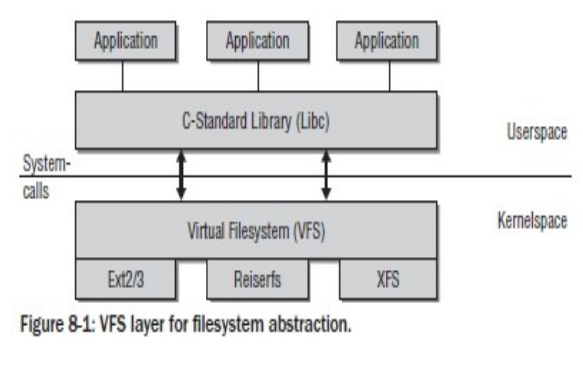
\includegraphics[scale=0.5]{capturas/1}
 \caption{Capa de abstracción del VFS \cite{diapo}} \label{fig:AQUI}
\end{figure}

\tab Cuando una aplicación accede a un sistema de archivos mediante una función, esta llamará al VFS independientemente del sistema de archivos al que se quiere acceder. El VFS transforma esta llamada a una llamada al sistema de ficheros interno, que a su vez se direcciona a una función de proyección del sistema de archivos concreto al que queramos acceder.\\

\tab Veámoslo gráficamente. En la figura \ref{figura 2} podemos ver como se interactuan los distintos módulos a través de los cuales una llamada al sistema de archivos por parte del usuario llega finalmente a dicho SA.que lanzará la llamada específica del sistema de archivos. \\

\begin{figure}[H]
  \centering
	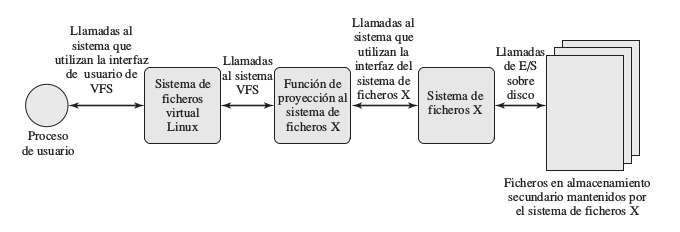
\includegraphics[scale=0.65]{capturas/funciones}
  \caption{Gráfico de comunicación entre los distintos módulos \cite{stalling}} \label{figura 2}
\end{figure} 

\section {Estructuras de datos \cite{kernel-doc}}

\tab Los VFS son orientados a objetos y constan de dos componentes, archivos y SA, que necesita gestionar y abstraer. \\

\tab Se representa a un archivo y a un SA con una familia de estructuras  de  datos hechas en C. Existen 4 tipos de objetos primarios del VFS:

\begin{enumerate}
	\item Objeto superblock
	\item Objeto inode
	\item Objeto dentry
	\item Objeto file
\end{enumerate}

\subsection {Objeto superblock} 

\tab Representa a un SA montado. El hecho de que esté montado y la información sobre el punto de montaje, así como diversos flags de montaje se almacena en la \emph{struct vfsmount}, cuya declaración se encuentra en \emph{linux/mount.h} \cite{silberschatz}: 

\begin{verbatim}
struct vfsmount {
  kdev_t mnt_dev;                       /* Device this applies to */
  char *mnt_devname;                    /* Name of device e.g. /dev/dsk/hda1 */
  char *mnt_dirname;                    /* Name of directory mounted on */
  unsigned int mnt_flags;               /* Flags of this device */
  struct super_block *mnt_sb;           /* pointer to superblock */
  struct quota_mount_options mnt_dquot; /* Diskquota specific mount options */
  struct vfsmount *mnt_next;            /* pointer to next in linkedlist */
};
\end{verbatim}



\tab Estas estructuras \emph{vfsmount} están unidas en una lista enlazada que comienza en \emph{vfsmntlist} en \emph{fs/super.c}. \\

\tab En cuanto al superbloque en sí, podemos encontrar su declaración en \emph{linux/fs.h}: 

\begin{verbatim}
struct super_block {
        struct list_head        s_list;         /* Keep this first */
        kdev_t                  s_dev;
        unsigned long           s_blocksize;
        unsigned char           s_blocksize_bits;
        unsigned char           s_lock;
        unsigned char           s_dirt;
        struct file_system_type *s_type;
        struct super_operations *s_op;
        struct dquot_operations *dq_op;
        unsigned long           s_flags;
        unsigned long           s_magic;
        struct dentry           *s_root;
        wait_queue_head_t       s_wait;

        struct inode            *s_ibasket;
        short int               s_ibasket_count;
        short int               s_ibasket_max;
        struct list_head        s_dirty;        /* dirty inodes */
        struct list_head        s_files;

        union {
                /* Configured-in filesystems get entries here */
                void                    *generic_sbp;
        } u;
        /*
         * The next field is for VFS *only*. No filesystems have any business
         * even looking at it. You had been warned.
         */
        struct semaphore s_vfs_rename_sem;      /* Kludge */
};
\end{verbatim}

\tab Estas son las operaciones que se pueden realizar sobre el superbloque: 

\begin{verbatim}
struct super_operations {
        void (*read_inode) (struct inode *);
        void (*write_inode) (struct inode *);
        void (*put_inode) (struct inode *);
        void (*delete_inode) (struct inode *);
        int (*notify_change) (struct dentry *, struct iattr *);
        void (*put_super) (struct super_block *);
        void (*write_super) (struct super_block *);
        int (*statfs) (struct super_block *, struct statfs *, int);
        int (*remount_fs) (struct super_block *, int *, char *);
        void (*clear_inode) (struct inode *);
        void (*umount_begin) (struct super_block *);
};
\end{verbatim}

\subsection {Objeto inode} 

\tab Una \emph{struct inode} representa un archivo de cualquier tipo (archivos, directorios, ...). El VFS no hace ninguna distinción entre tipos de objetos, deja esta tarea en manos de níveles del kernel más altos. \\

\tab Cada inodo está representado por una de estas structs, \emph{struct inode}, y puede realizar una serie de métodos almacenados en \emph{struct inode\_operations}. \cite{stalling} \\

\begin{verbatim}
struct inode {
        struct list_head        i_hash;
        struct list_head        i_list;
        struct list_head        i_dentry;

        unsigned long           i_ino;
        unsigned int            i_count;
        kdev_t                  i_dev;
        umode_t                 i_mode;
        nlink_t                 i_nlink;
        uid_t                   i_uid;
        gid_t                   i_gid;
        kdev_t                  i_rdev;
        off_t                   i_size;
        time_t                  i_atime;
        time_t                  i_mtime;
        time_t                  i_ctime;
        unsigned long           i_blksize;
        unsigned long           i_blocks;
        unsigned long           i_version;
        unsigned long           i_nrpages;
        struct semaphore        i_sem;
        struct inode_operations *i_op;
        struct super_block      *i_sb;
        wait_queue_head_t       i_wait;
        struct file_lock        *i_flock;
        struct vm_area_struct   *i_mmap;
        struct page             *i_pages;
        spinlock_t              i_shared_lock;
        struct dquot            *i_dquot[MAXQUOTAS];
        struct pipe_inode_info  *i_pipe;

        
        unsigned long           i_state;

        unsigned int            i_flags;
        unsigned char           i_sock;

        atomic_t                i_writecount;
        unsigned int            i_attr_flags;
        __u32                   i_generation;
        union {
                ....
                struct ext2_inode_info          ext2_i;
                ....
                struct socket                   socket_i;
                void                            *generic_ip;
        } u;
};
\end{verbatim}

\tab A lo largo de la asigntura, tanto en la parte práctica como en la teórica, hemos hecho referencia a algunas de estos elementos, como pueden ser \emph{i\_ino}, \emph{i\_count}, \emph{umode\_t i\_mode}, \emph{struct inode\_operation}...

\subsection{Objeto dentry}

\tab Cada uno de estos objetos representa una entrada de directorio (directory entry - dentry). Este tipo de objetos tienen como objetivo entre otras cosas relacionar un objeto de tipo inodo con uno de tipo file utilizando el número de inodo y el nombre del file. También ayudan a mantener de forma eficiente los archivos usados frecuentemente. Al igual que el superbloque y el inodo, los métodos que se pueden utilizar con los objetos de tipo dentry se almacenan en \emph{struct dentry\_operations}.

\begin{verbatim}
struct dentry {
        int d_count;
        unsigned int d_flags; 
        struct inode  * d_inode;        /* Where the name belongs to - NULL is negative */
        struct dentry * d_parent;       /* parent directory */
        struct dentry * d_mounts;       /* mount information */
        struct dentry * d_covers;
        struct list_head d_hash;        /* lookup hash list */
        struct list_head d_lru;         /* d_count = 0 LRU list */
        struct list_head d_child;       /* child of parent list */
        struct list_head d_subdirs;     /* our children */
        struct list_head d_alias;       /* inode alias list */
        struct qstr d_name;
        unsigned long d_time;           /* used by d_revalidate */
        struct dentry_operations  *d_op;
        struct super_block * d_sb;      /* The root of the dentry tree */
        unsigned long d_reftime;        /* last time referenced */
        void * d_fsdata;                /* fs-specific data */
        unsigned char d_iname[DNAME_INLINE_LEN]; /* small names */
};
\end{verbatim}

\subsection{Objeto file}

\tab Al contrario que las estructuras anteriores que tenían una instancia al nivel del sistema, las \emph{struct file} son estructuras creadas a nivel de proceso. Una vez todos los procesos que utilizaban el archivo abierto terminan esta struct es desechada. Almacenará información sobre el contenido del archivo, su estado, donde está el archivo en sí y los procesos que lo están usando (el ya clásico \emph{f\_count} que mantendrá el número de procesos que están usando el archivo. Si llega a tomar el valor 0, la struct se destruye). \cite{diapo} \\

\tab Del mismo modo que se hizo con los objetos anteriores, los métodos de este objeto se almacenan en \emph{struct file\_operations}. \\

\begin{verbatim}
struct file {
   struct list_head         f_list;
   struct dentry            *f_dentry;
   struct file_operations   *f_op;
   atomic_t                 f_count;
   unsigned int             f_flags;
   mode_t                   f_mode;
   loff_t                   f_pos;
   unsigned long            f_reada, f_ramax, f_raend, f_ralen, f_rawin;
   struct fown_struct       f_owner;
   unsigned int             f_uid, f_gid;
   int                      f_error;

   unsigned long            f_version;

   /* needed for tty driver, and maybe others */
   void                     *private_data;
\};
\end{verbatim}

\section{Uso de memoria}

\tab En este aspecto el VFS utiliza directamente algunas de las cachés mencionadas en la asignatura y otras no estudiadas. Entre ellas están las cachés de i-nodos y de directorios (dentry). \\

\tab Es importante no confundir estas cachés con la caché física en el sentido de que estas residen en memoria principal y almacenan structs de un tipo específico cada una. \\

\tab De esta forma, cuando un i-nodo es referenciado por primera vez, se copia su información a la caché de i-nodos (en memoria principal), para que las referencias que se realicen a continuación sean más rápidas. \\

\tab Una vez eliminamos una struct de la caché, las correspondientes entradas son marcadas como "libres". El VFS reutiliza estas entradas realizando procesos de asignación de memoria solo cuando no tiene entradas libres. Esto se implenta mediante listas encadenadas de structs libres. En comparación con una operación de asignación o liberación de memoria, este proceso es mucho menos costoso, aumentando así el rendimiento. \cite{politecnica} \\

\begin{figure}[H]
  \centering
 	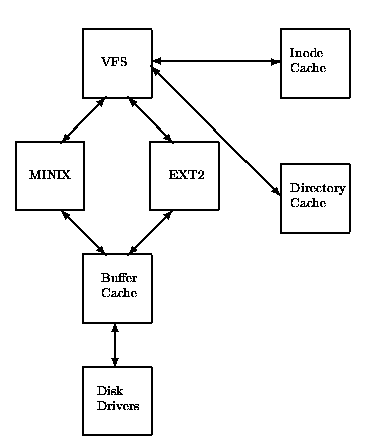
\includegraphics[scale=0.65]{capturas/cache}
 	\caption{Diagrama lógico del VFS \cite{trento}} \label{fig:YA AQUI}
\end{figure}

\section{Conclusión}

\tab El VFS de Linux lo convierte en un sistema operativo muy versátil en cuanto a sistemas de archivos se refiere. Podemos utilizar con la misma facilidad prácticamente cualquier sistemas de archivos gracias a la capa de abstracción implementada. Por otro lado vamos a perder velocidad ya que obviamente es más lento realizar llamadas al VFS y los módulos de proyección intermedios frente a dirigirse directamente al sistema de archivos concreto. \cite{carretero} \\

\tab Frente a esta versatilidad, otros sistemas operativos no ofrecen soporte para tantos sistemas de archivos, centrándose más en otros ámbitos como la eficiencia. Un ejemplo de ello es Windows, quien además de soportar varios sistemas de archivos tiene implementado uno propio, el sistema de ficheros de Windows (NTFS), pensado para alcanzar requisitos de altas prestaciones en estaciones de trabajo y servidores. \cite{stalling} \\ 

\bibliographystyle{plain}
\bibliography{citas}


\end{document}